\part{Scholarly literature}
\frame{\partpage}

\begin{frame}{Scholarly work}
	\begin{itemize}
		\pause\item What is a ``scholarly'' work?
		\pause\item How do we know if something is scholarly?
	\end{itemize}
\end{frame}

\usetikzlibrary{shapes,arrows,intersections}
\usetikzlibrary{matrix,fit,calc,trees,positioning,arrows,chains,shapes.geometric,shapes}

\begin{frame}{Pyramid of sources}
	\centering
	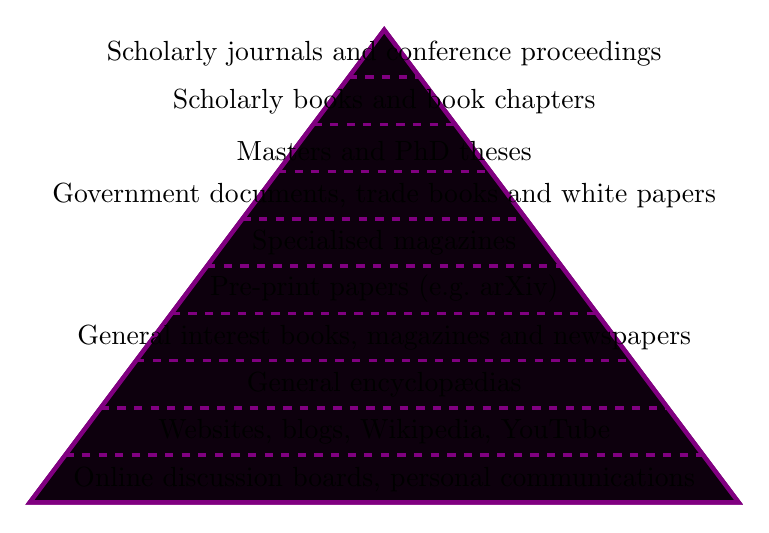
\begin{tikzpicture}
	\coordinate (A) at (-4.5,0) {};
	\coordinate (B) at ( 4.5,0) {};
	\coordinate (C) at (0,5*1.2) {};
	\path[name path=AC,draw=none] (A) -- (C);
	\path[name path=BC,draw=none] (B) -- (C);
	\iftoggle{printable}{
		\filldraw[draw=Purple, ultra thick,fill=Purple!10!White] (A) -- (B) -- (C) -- cycle ;
	}{ % else
		\filldraw[draw=Purple, ultra thick,fill=Purple!10!Black] (A) -- (B) -- (C) -- cycle ;
	}	

	\foreach \y/\A in {4.5/{Scholarly journals and conference proceedings},
					   4.0/{Scholarly books and book chapters},
					   3.5/{Masters and PhD theses},
					   3.0/{Government documents, trade books and white papers},
					   2.5/{Specialised magazines},
					   2.0/{Pre-print papers (e.g.\ arXiv)},
					   1.5/{General interest books, magazines and newspapers},
					   1.0/{General encyclop\ae dias},
					   0.5/{Websites, blogs, Wikipedia, YouTube},
					   0.0/{Online discussion boards, personal communications}
					} {
		\pause
		\path[draw=none, very thick, dashed, name path=horiz] (A|-0,\y*1.2) -- (B|-0,\y*1.2);
		\draw[draw=Purple, very thick, dashed, 
			  name intersections={of=AC and horiz,by=P},
			  name intersections={of=BC and horiz,by=Q}] (P) -- (Q)
			  %node[midway,above,font=\bfseries\scshape,color=red!60!Brown] {\A};
			  node[midway,above] {\A};
	}
	\end{tikzpicture}
\end{frame}

\begin{frame}{Appropriateness of sources}
	\pause It is important to question the \textbf{appropriateness} of sources you use in academic work
	\begin{itemize}
		\pause\item \textbf{Validity}: Are claims based upon a correct interpretation of the evidence?
		\pause\item \textbf{Rigor}: Was the method of collecting evidence appropriate to ensure 
			comprehensive coverage while also avoiding bias?
	\end{itemize}
\end{frame}

\begin{frame}{Appropriateness of sources}
	\begin{itemize}
		\pause\item \textbf{Reliability}: has the claim been replicated, or at least reviewed, by other academics?
		\pause\item \textbf{Authoritativeness}: do we know who the author is?
			Does the author have enough experience in the field to present a fair and balanced argument?
		\pause\item \textbf{Venue}: Is the publisher reputable and free of undue editorial influences?
	\end{itemize}
\end{frame}

\begin{frame}{Appropriateness of sources}
	\pause There are of course exceptions where sources are presented as \textbf{artefacts} and/or \textbf{archives}:
	\begin{itemize}
		\pause\item Citing a newspaper as evidence for a claim based on the reception of a new technology
		\pause\item Citing a manufacturer's technical manual when describing a technical feature of a platform
		\pause\item Citing a Reddit post by a well-known industry figure as evidence for expert opinion
	\end{itemize}
	\pause The \textbf{way} in which sources are \textbf{used} is therefore important
\end{frame}
